\documentclass[12pt,
paper=a4,				
DIV=calc,		  % führt die Satzspiegelberechnung neu aus
%oneside,		  % einseitiger Druck
BCOR=16mm,	  % Bindekorrektur
headinclude,
%footinclude,
openany
]{scrbook}


%****************
% define medatata
%________________
\def\Title{An Example Document}
\def\Author{Some Name}
\def\Subject{An Example Document}
\def\Keywords{LaTeX,Example,Document}
 
%***************************************************************************
% \convertDate converts D:20080419103507+02'00' to 2008-04-19T10:35:07+02:00
%___________________________________________________________________________
\def\convertDate{%
    \getYear
}
 
{\catcode`\D=12
 \gdef\getYear D:#1#2#3#4{\edef\xYear{#1#2#3#4}\getMonth}
}
\def\getMonth#1#2{\edef\xMonth{#1#2}\getDay}
\def\getDay#1#2{\edef\xDay{#1#2}\getHour}
\def\getHour#1#2{\edef\xHour{#1#2}\getMin}
\def\getMin#1#2{\edef\xMin{#1#2}\getSec}
\def\getSec#1#2{\edef\xSec{#1#2}\getTZh}
\def\getTZh +#1#2{\edef\xTZh{#1#2}\getTZm}
\def\getTZm '#1#2'{%
    \edef\xTZm{#1#2}%
    \edef\convDate{\xYear-\xMonth-\xDay T\xHour:\xMin:\xSec+\xTZh:\xTZm}%
}
 
\expandafter\convertDate\pdfcreationdate 
 
%**************************
% get pdftex version string
%__________________________
\newcount\countA
\countA=\pdftexversion
\advance \countA by -100
\def\pdftexVersionStr{pdfTeX-1.\the\countA.\pdftexrevision}
 
 
%*********
% XMP data
%_________
\usepackage{xmpincl}
%\includexmp{pdfa-1b}
 
%********
% pdfInfo
%________
\pdfinfo{%
    /Title    (\Title)
    /Author   (\Author)
    /Subject  (\Subject)
    /Keywords (\Keywords)
    /ModDate  (\pdfcreationdate)
    /Trapped  /False
}
 


\usepackage[utf8]{inputenc}
\usepackage{color}
\usepackage{graphicx}
\setcapindent{1em}
%\usepackage{wrapfig}
\usepackage{sidecap}

\bibliographystyle{alpha} 
\newcommand{\fett}[1]{{\bf #1}}
\newcommand{\TODO}[1]{{\LARGE{\textcolor{red}{\emph {#1 }}}}}
\clubpenalty10000
\widowpenalty10000

\makeindex
\begin{document}

\titlehead{Friedrich Schiller Universität Jena\\
PAF}
\subject{Dissertation}
\title{High-Fluence Ion Beam Irradiation of Semiconductor Nanowires}
\author{Andreas Johannes}
\date{July 2015}
\maketitle






\tableofcontents

\chapter{Introduction}
\pagenumbering{arabic}
\setcounter{page}{1}
%\let\clearpage\relax




%We are living in an era dominated by the information technology. There is virtually no part of life not influenced by the continuing advances in the digital world and semiconductors, especially silicon, are at the base of each and every logic unit dealing in `ones' and `zeros'. Silicon therefore quickly became one of the most studied materials, catching up with the previously dominating iron and its various alloys with other elements, steel.

Technological progress generally shows a competition between the optimization of the dominating technology and the development of fundamentally new operation principles. An example of this competition is recorded in the ``International Technology Roadmap for Semiconductors'', which aims to guide the scaling of digital devices to follow ``Moore's Law'' of improved performance, and the white paper ``Towards a `More-than-Moor' roadmap'', which examines opportunities to include non-digital functionality where performance does not necessarily have to scale with size. Both are available at the ITRS website  \cite{map_http://www.itrs.net/_2015}. A shift in operating principle is found, for example, in data storage, which changed fundamentally when the effect of giant magneto-resistance (GMR) was discovered in 1988. 
This quickly formed the basis for the standard hard-drives (HDD) and HDDs soon dominated PC data storage. Nowadays, the much older principle of flash memory is making a come-back in solid state drives (SSD), which begin to replace HDDs. They owe their viability (cost, speed and storage density) almost entirely to the advanced miniaturization, allowing the production of a floating gate for a transistor on a scale down to tens of nanometers per single $bit$, while producing \emph{billions} of $\nicefrac{bits}{cm^{2}}$. This shows, that it is not \emph{a priori} possible to discern with certainty which approach is going to produce the best results, so that much room is left for open minded fundamental research in general and on semiconductors in particular.

In the wake of the miniaturization used for the improvement of IT hardware technology, the new, multi-disciplinary field of nanotechnology has emerged. The scope of the field is illustrated by the high number of journals dedicated to research at the nanoscale. This includes semiconductor science, but in the leading journals \emph{ACS Nano} \cite{acs_nano_http://pubs.acs.org/journal/ancac3_2015}, \emph{Advanced Materials} \cite{advanced_materials_http://www.advmat./_2015}, \emph{Advanced Functional Materials} \cite{advanced_functional_materials_http://onlinelibrary.wiley.com/journal/10.1002/issn1616-3028_2015}, \emph{Nano Letters} \cite{nano_letters_http://pubs.acs.org/journal/nalefd_2015}, \emph{Nature Nanotechnology} \cite{nature_nanotechnology_http://www.nature.com/nnano_2015}, \emph{Nano Today} \cite{nano_today_http://journals.elsevier.com/17480132/nano-today/_2015}, \emph{Nanotoxicology} \cite{nanotoxicology_http://www.informahealthcare.com/nan_2015}, \emph{Small} \cite{small_http://www.small-journal.com/_2015} and others, fundamental research and applications of nanoscale devices and effects from all natural sciences are published.

The specific class of nanomaterials investigated in this thesis are semiconductor nanowires, which have gained a significant amount of  interest \cite{huang_room-temperature_2001,cui_nanowire_2001,duan_indium_2001,xia_one-dimensional_2003,lieber_functional_2007}. `Nanowire' is a term used for many morphologies, but it seems a reasonable name for structures with a cross-section that is between $1 \times 1$ and $1000 \times 1000\,nm^2$ and a large length to form a high aspect ratio. One of the general aspects of this shape and also of nanostructured materials in general, is that the surface properties play a dominating role. This is simply caused by the fact, that there is a lot of surface per volume of material. As the surface to volume ratio in general is proportional to $1/r$ for a body with a characteristic constraining length of $r$, it gets very large for small structure sizes.

The wire shape has an inherent advantage over three dimensionally constrained particles (nanoclusters, quantum dots etc.), in that it is easier to define contacts and drive a current through a nanoscale wire than through a nanoscale dot. Incidentally, the idea to combine this specific advantage of nanowires with new properties obtained by the stronger three dimensional confinement of quantum dots is the main idea behind the `Deutsche Forschungsgemeinschaft' (DFG) project ``wiring quantum dots", which funded this work. 

The defining property of semiconductors is the ability to dramatically change their electronic properties by adding impurities \cite{sze_physics_2006}. As ion beam irradiation can be used to `mix' (i.e. dope) virtually any target material with a precisely controlled number of atoms of practically any element, it was and is a key part in the processing and development of semiconductor technologies. 

In general, ion beam doping has the advantage over doping during the synthesis of nanostructures, since it is not inherently limited by the chemical potentials and thermodynamics which typically have to be carefully controlled for the synthesis of nanostructures. It is a non-equilibrium physical process by which different elements can forcefully be introduced into a target matrix with much higher energies than those involved in chemical bonding. The extent of disorder created in the target during this bombardment, whether the intermixing is thermodynamically stable and whether a desired (crystalline) order can be reestablished by thermal annealing is in the focus of ion-beam physics. A good background on this can be gained from dedicated literature \cite{ziegler_stopping_1985,eckstein_computer_1991,nastasi/mayer/hirvonen_ion-solid_2008,schmidt_ion_2012}.

%Scaling down material to the nanoscale becomes interesting when the structure size reaches the characteristic dimension of the effect governing the physical properties of interest. Then new, mesoscopic and quantum mechanical properties can emerge. As an example, the changed light-matter interaction in structures of the dimension of the wavelength of light is investigated in the field of nano-photonics and plasmonics \cite{saleh_fundamentals_2007,maier_plasmonics:_2007}.


Typical ion ranges for the doping of semiconductors lie in the range of $10$-$100\,nm$. Therefore, ion beam irradiation of nanostructures of the same dimension will show some interplay between the irradiated structures' dimensions and the ion range. The many practical applications of the combination of ion beams and nanostructures warrants general investigations of the nanostructure - ion beam interaction and the topic has therefore gained increased interest very recently \cite{borschel_ion-solid_2012,greaves_enhanced_2013,nietiadi_sputtering_2014,johannes_ion_2015,urbassek_sputter_2015}.  

A specific example in which the combination of nanostructures and ion beams is advantageous is the ion irradiation of diamond to create nitrogen-vacancy clusters. The diamond is nanostructured to facilitate efficient extraction of light, while ion irradiation with nitrogen creates nitrogen-vacancy clusters very effectively. These are interesting as promising components in a future quantum information device \cite{babinec_diamond_2010}. The precise control ion irradiation gives, makes it possible to implant a well defined number of ions with reasonable spacial accuracy. This control is extravagantly demonstrated by the possibility of single ion irradiation, shown in references \cite{meijer_concept_2006,ohdomari_single-ion_2008}. 

In addition to this extremely low ion fluence example of ion irradiation, the next two examples of the concurrence of nanotechnology and ion-irradiation led more or less directly into the investigations into high fluence irradiation presented in this dissertation. Firstly there is the search for a diluted magnetic semiconductor for which $Mn$ doped $GaAs$-nanowires are a good candidate. As $GaAs$ nanowires typically grow above $450^\circ C$ but $MnAs$ segregates from $Ga_{(1-x)}Mn_xAs$ at around $350^\circ C$ \cite{dietl_engineering_2006,sadowski_gaasmnas_2011}, there is no straightforward way to dope $GaAs$-nanowires with high concentrations of $Mn$ during their growth. However, it can be achieved by implanting $Mn$ in $GaAs$-nanowires. Best results are achieved when the irradiation is performed at elevated temperatures, hot enough to minimize disorder introduced by the ion beam, but cold enough to prevent segregation of $MnAs$ \cite{borschel_new_2011,paschoal_hopping_2012,borschel_ion-solid_2012,kumar_magnetic_2013,paschoal_magnetoresistance_2014}. 

Conversely, the ``wiring quantum dots'' project aimed to utilize the segregation of ion-implanted material in a nanowire to form nanowires decorated with nanoclusters. When $Si$ nanowires are irradiated with high fluences of $In^+$ and $As^+$ and subsequently annealed with a flash-lamp, separated $InAs$ slices form within the $Si$ nanowires \cite{prucnal_iii-v_2014,glaser_personal_2015}. The supersaturation of $Si$ with $In$ and $As$ by ion implantation can thus be utilized to create $Si$-$InAs$ nanowire hetero-structures from a $Si$ nanowire template in a relatively straightforward manner.
 
A further important example of the intersection of nanotechnology and ion beams is found in the ubiquitous focused ion beam (FIB) systems. The production and development of many of the novel nanoscale devices on the horizon often requires the precise ion beam milling that FIBs provide with a resolution of few nanometers \cite{kranz_integrating_2001,george_nanopore_2010,chalapat_self-organized_2013}. In all the examples given so far, and virtually per definition in the last one, the typical structure sizes irradiated are in the same order of magnitude at the range of the impinging ions. Understanding how this affects the ion-matter interaction can be crucial to the successful outcome of the respective experiments.

In the effort to understand principles and fundamental interactions on the nanometer length scales, nanowires are a very good model system to investigate, as their geometry is fully characterized by their height and radius. Spheres, which would have a degree of freedom less, are more difficult to handle, as the unavoidable proximity of a substrate may influence their behavior \cite{hu_burrowing_2002,klimmer_size-dependent_2009,moller_tri3dyn_2014,johannes_ion_2015}. The understanding of the ion-nanostructure interaction gained by investigating irradiated nanowires is principally transferable to any nanostructure. However, this can hardly be done in any general way explicitly, as the possible shapes of nanostructures are uncountable. This dissertation adds to the growing field of nanostructure - ion beam interaction the discussion of three effects which are especially important in high fluence irradiation and dedicates a separate chapter to each. 
 
\begin{description}
  \item[\normalfont Chapter 3 - Sputtering of Nanowires] \hfill \\
  In the dissertation of Dr. C. Borschel \cite{borschel_ion-solid_2012} the program \emph{iradina} \cite{borschel_ion_2011} was developed and used to simulate the ion irradiation of nanostructures. It predicts an enhanced, diameter-dependent sputter yield in nanostructures. This chapter discusses the simulation and compares its predictions with experimentally obtained diameter-dependent sputtering in nanowires. Some first results on the sputtering during $Mn$ irradiation of $GaAs$-nanowires are published elsewhere \cite{johannes_enhanced_2014}. The results presented here are on $Ar$ irradiated $Si$-nanowires. They were obtained in close cooperation with Stefan Noack \cite{noack_sputter_2014} in his M.Sc. and also published in reference \cite{johannes_anomalous_2015}.
  \item[\normalfont Chapter 4 - High Doping Concentrations in Nanowires] \hfill \\
  The concentration of dopants does not follow a linear increase with the fluence of ions implanted for high fluences. It has already been observed that sputtering of the target will dynamically change its composition during the ion irradiation in addition to the intended change by incorporation of the ions within the target material \cite{moller_tridyn_1984,moller_tridyn-binary_1988,miyagawa_computer_1991,sigmund_alloy_1993,eckstein_oscillations_2000}. This effect is enhanced in nanostructures, first, since the sputtering is enhanced when compared to bulk samples as shown in the preceding chapter, but also since there is simply less material. Hence, the effect of removing material by sputtering already becomes significant at lower fluencies in nanostructures than in bulk. The presented results are acquired by compositional analysis using nano-XRF performed on 175\,keV Mn$^+$ ion irradiated ZnO nanowires \cite{johannes_enhanced_2014}. They are discussed in comparison to a pseudo-dynamic simulation performed using results from \emph{iradina}.
  \item[\normalfont Chapter 5 - Plastic Flow in Silicon Nanowires] \hfill \\
  In the high ion fluence irradiated $Si$ nanowires an unexpected tendency of the nanowires to become shorter was observed. This chapter presents a dedicated investigation into this plastic deformation of $Si$ under ion irradiation which has been previously seen only in high energy ($\ge\,MeV$) ion irradiations \cite{volkert_stress_1991,trinkaus_viscoelastic_1995,hedler_amorphous_2004,hedler_boundary_2005}.
\end{description}



\chapter{Methods}


Ausgiebige Verwendung von \emph{iradina} \cite{borschel_ion_2011}

\chapter{Sputtering of Nanostructures}


When an energetic ion hits a solid target the ensuing collision cascade will displace some of the target atoms from their original positions. The energy lost by the ion in these collisions is called ``nuclear'' energy loss. A displaced target atom can either become an interstitial, if it stays within the target volume, or be sputtered if it has sufficient energy to leave the solid. The energy required to leave the target is the surface-binding-energy.

\chapter{High Doping Concentrations in Nanostructures}


\chapter{Plastic Flow in Nanostructured Silicon}

It was mentioned before that within the ``wiring quantum dots'' project $Si$ nanowires where irradiated with $As^+$ and $In^+$ and/or $Ga^+$ so that in a subsequent annealing step $Si-GaAs$ or $Si-InGaAs$ hetero-structures could be formed. Markus Glaser the Ph.D. student responsible for this part of the project had developed a good habit of making SEM images of the same individual wires after each process step. We thus noticed, that the $Si$ nanowires shrank quite dramatically during the irradiation with $\approx 100\,keV$ $In^+$, $Ga^+$ and $As^+$ at room temperature. Two examples of this can be seen in figure \TODO{Figure}\ref{deformSEM}. A quick look into literature revealed that this behavior has not been observed at such low ion energies. A thorough investigation might be worthwhile. Similar $Si$ nanowire arrays as the ones used for the sputtering experiment were thus systematically irradiated with $Ar^+$ to avoid any chemical effects, making SEM images after each irradiated fluence to observe and quantify the deformation.

\begin{SCfigure}
	\centering
		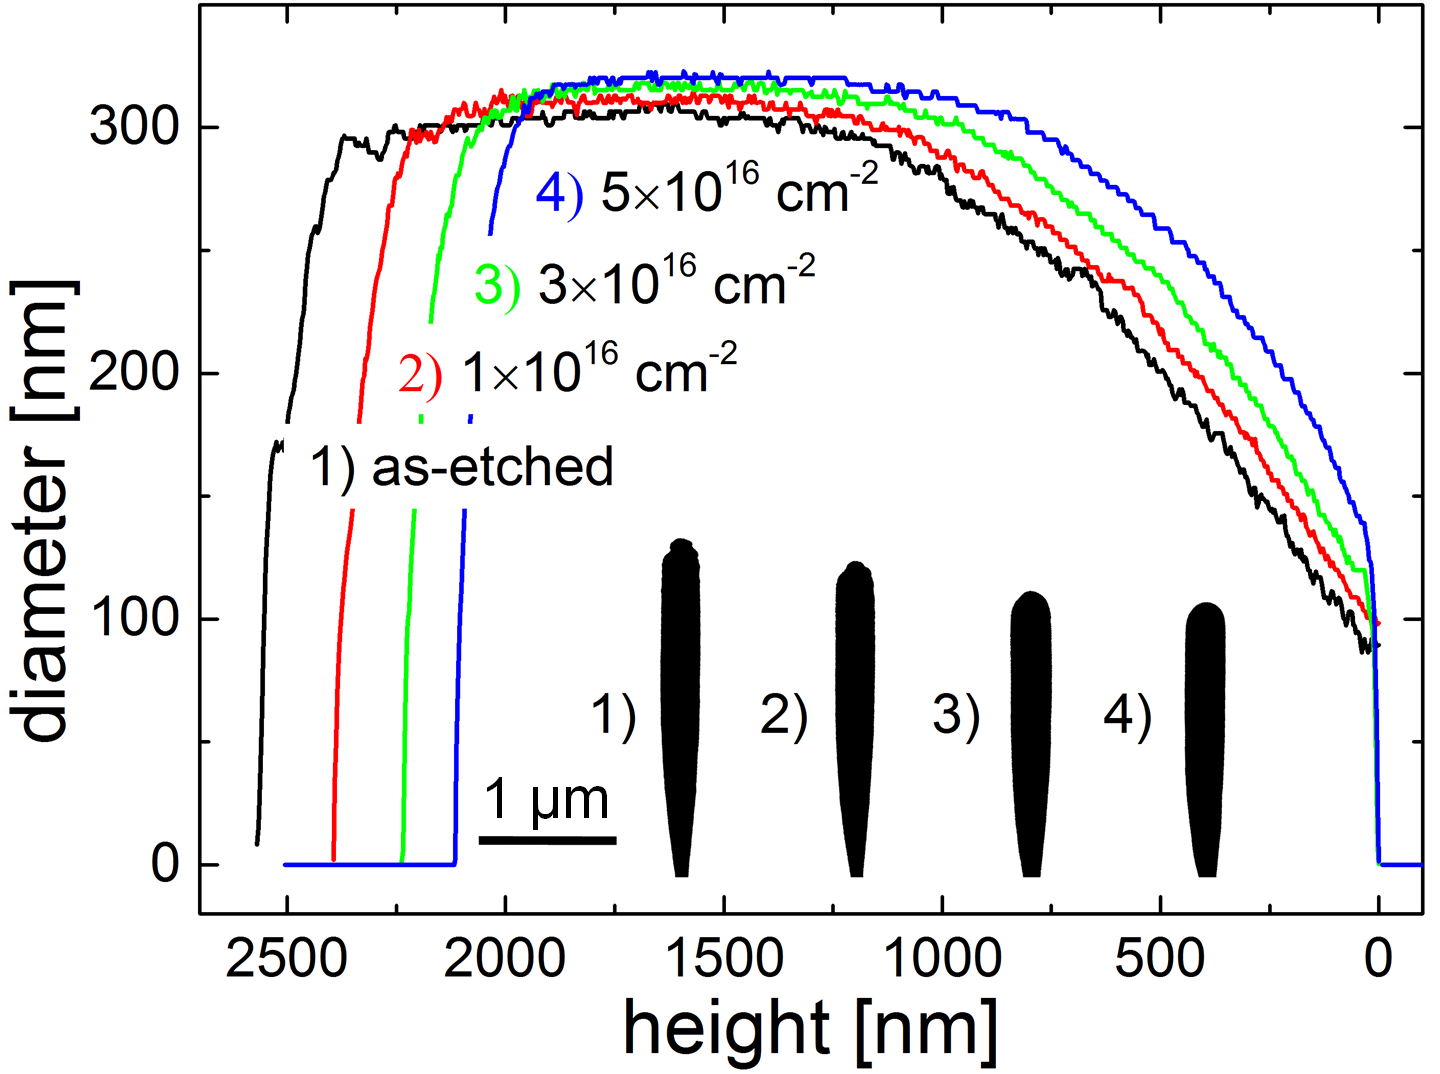
\includegraphics[width=.48\textwidth]{images/deformationprofile.jpg}
	\caption{Graphs of the diameter over height of a single $Si$ nanowire irradiated with increasing fluences of $100\,keV Ar^+$ ions. The black insets show the profiles of the nanowire after the respective fluences extracted from SEM images. In both illustrations the shrinking and widening of the wire is clearly visible.} 
	\label{deformationprofile}
\end{SCfigure}

Using the algorithm described in the sputter yield chapter, the profiles for the irradiated nanowires could be extracted. In figure \ref{deformationprofile} the black, red, green and blue lines indicate the height dependent diameter of a single wire before and after irradiation with $100\,keV Ar^+$ up to fluences of 1, 3 and $5 \times 10^{16}\,cm^{-2}$ respectively. In this graph, as well as in the inset black profiles, the reduction of the height by $\approx 500\,nm$ and an increase of the diameter, especially at the base, can be clearly seen.

In the collision cascade following an energetic ion impinging a solid will preferentially knock-on atoms along the propagation direction of the impinging ion. This causes an inhomogeneous distribution of interstitials and vacancies and effectively mass is transported `downstream' along the ion beam. In an amorphous material it is not clear what constitutes an `interstitial' or a `vacancy', but a local excess of vacancies can be understood as a locally decreased density, while an interstitial excess corresponds to an increased density. A local density gradient is not stable, since the density of amorphous $Si$ before and after irradiation is not significantly different \cite{pelaz_ion-beam-induced_2004}. Therefore the density gradient introduces stress in the material which can relax by plastic deformation, possibly enabled by a decreased viscosity due to further ion irradiation. 

As it was shown in the previous chapters that the BCA simulation software can accurately reproduce the collision cascades, let us see whether the deformation observed in the experiment can be accounted for with this knock-on mass transport. Figure \ref{deformationBCA}a) shows the simulation volume implemented in \emph{iradina} with $2\times2\times2\,nm^3$ voxels as a $600\,nm$ long $Si$ cylinder with a diameter of $200\,nm$. The $100\,keV\,\,Ar^+$ ions impinge at an angle of $45^\circ$ to the $z$-axis. They striking the cylinder distributed uniformly along the $y$-direction at height $z=0$. Figure \ref{deformationBCA}d) shows the resulting distribution of interstitials on the cross-sectional slice through the middle of the nanowire along the $xz$ plane. This can be seen as an approximation for the distribution of the nuclear energy loss and shows the mean extent of collision cascade. Figure \ref{deformationBCA}e)shows the same cross-section after subtracting the distribution of the vacancies. The excess of vacancies along the impinging plane (blue line in the cross section) enveloped by two red planes of excess interstitials shows that there is a high probability for the ions to hit a target atom with a large impact parameter. This changes the ions path only little and displaces the target atom in an direction perpendicular to the ion beam. Superimposing many collisions along the y direction leads to the formation of two interstitial rich and one vacancy rich planes. The $xy$-plane in \ref{deformationBCA}b) shows the sum over the height $z$ of the difference between interstitials and vacancies plotted to the same color scale. The illustration is dominated by vacancies at the surface of the cylinder which are left behind by sputtered atoms. 

The height distribution (summing over the radial $xy$ plane) of the interstitials, vacancies and leaving atoms is shown in \ref{deformationBCA}c). As expected, the majority of sputtered atoms originate near the impact height. The lines showing the interstitials and vacancies overlap in this illustration. Subtracting the vacancies from the sum of interstitials and leaving atoms and their the distribution along the height is plotted in f). As a displaced atom which is either sputtered or becomes an interstitial always leaves behind a vacancy, the sum over all heights of this plot is zero. The strong oscillation around $z=0$ is caused by the previously discussed perpendicular displacement of target atoms for large impact parameters. This oscillation is very sensitive to the voxel-size as interstitial and vacancy rich regions are superimposed for larger voxels. The excess of vacancies near the impact point ($\le 70\,nm$) and of interstitials further down along the ion's path ($\approx 100\,nm$) is not sensitive to the voxel size. It can be used to quantify the knock-on mass transport by multiplying the plotted values by their height and integrating over all heights. At this point the influence of the short range oscillation immediately around the impact point disappears as here $z$ is small. The value obtained from this analysis is $78\pm1\,atoms \cdot nm /ion$.


BCA software typically checks at each collision whether the target atom acquires more energy than the ``displacement energy'' which is a material specific parameter. If the displaced atoms has less than the displacement energy, it is assumed, that it remains bound in its place, and that the energy is converted into lattice vibrations ($=$ heat).


\clearpage
\begin{figure}[htbp]
	\centering
		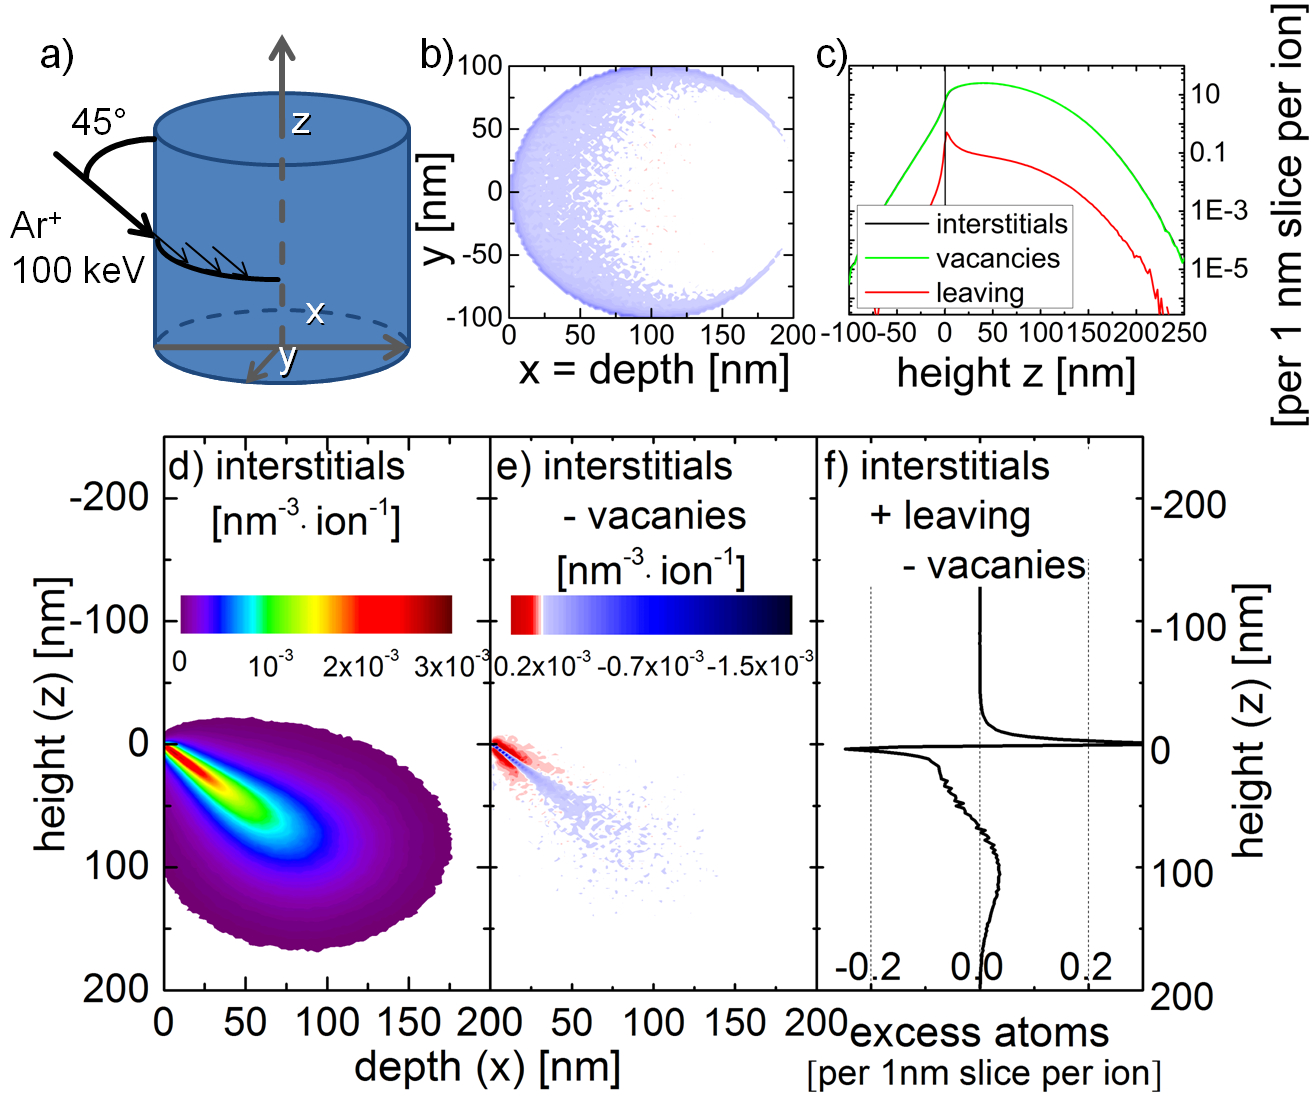
\includegraphics[width=.9\textwidth]{images/deformationBCA.jpg}
		\caption{a) Illustration of the simulated irradiation geometry. All $Ar^+$ ions of $100\,keV$ energy hit the nanowire volume at the same height and at an angle of $45^\circ$ with respect to the wire axis $z$. The created interstitials in the radial cross-section through the middle of the simulated nanowire is shown in d). This distribution is effectively an illustration of the nuclear energy loss. In e) the vacancies are subtracted from the interstitials for the same cross-section. Summing this difference over all heights gives the radial distribution shown in b). The clear dominance of vacancies near the surface is caused by sputtering. The axial profile of the interstitials, vacancies and leaving (sputtered) atoms plotted in c) over the height relative to the impact plane shows, that most atoms are sputtered at the impact height. Note that the plots of vacancies and interstitials overlap. The vacancies subtracted from the sum of interstitials and sputtered atoms plotted over the height in f) shows mass transport along the ions path. Apart from the strong oscillation at the impact height, there is a deficiency of atoms close to the impact height ($\le 70\,nm$) and an excess centered around $100\,nm$ down from the impact height.} 
	\label{deformationBCA}	
\end{figure}

\clearpage
test



\begin{figure}[htbp]
	\centering
		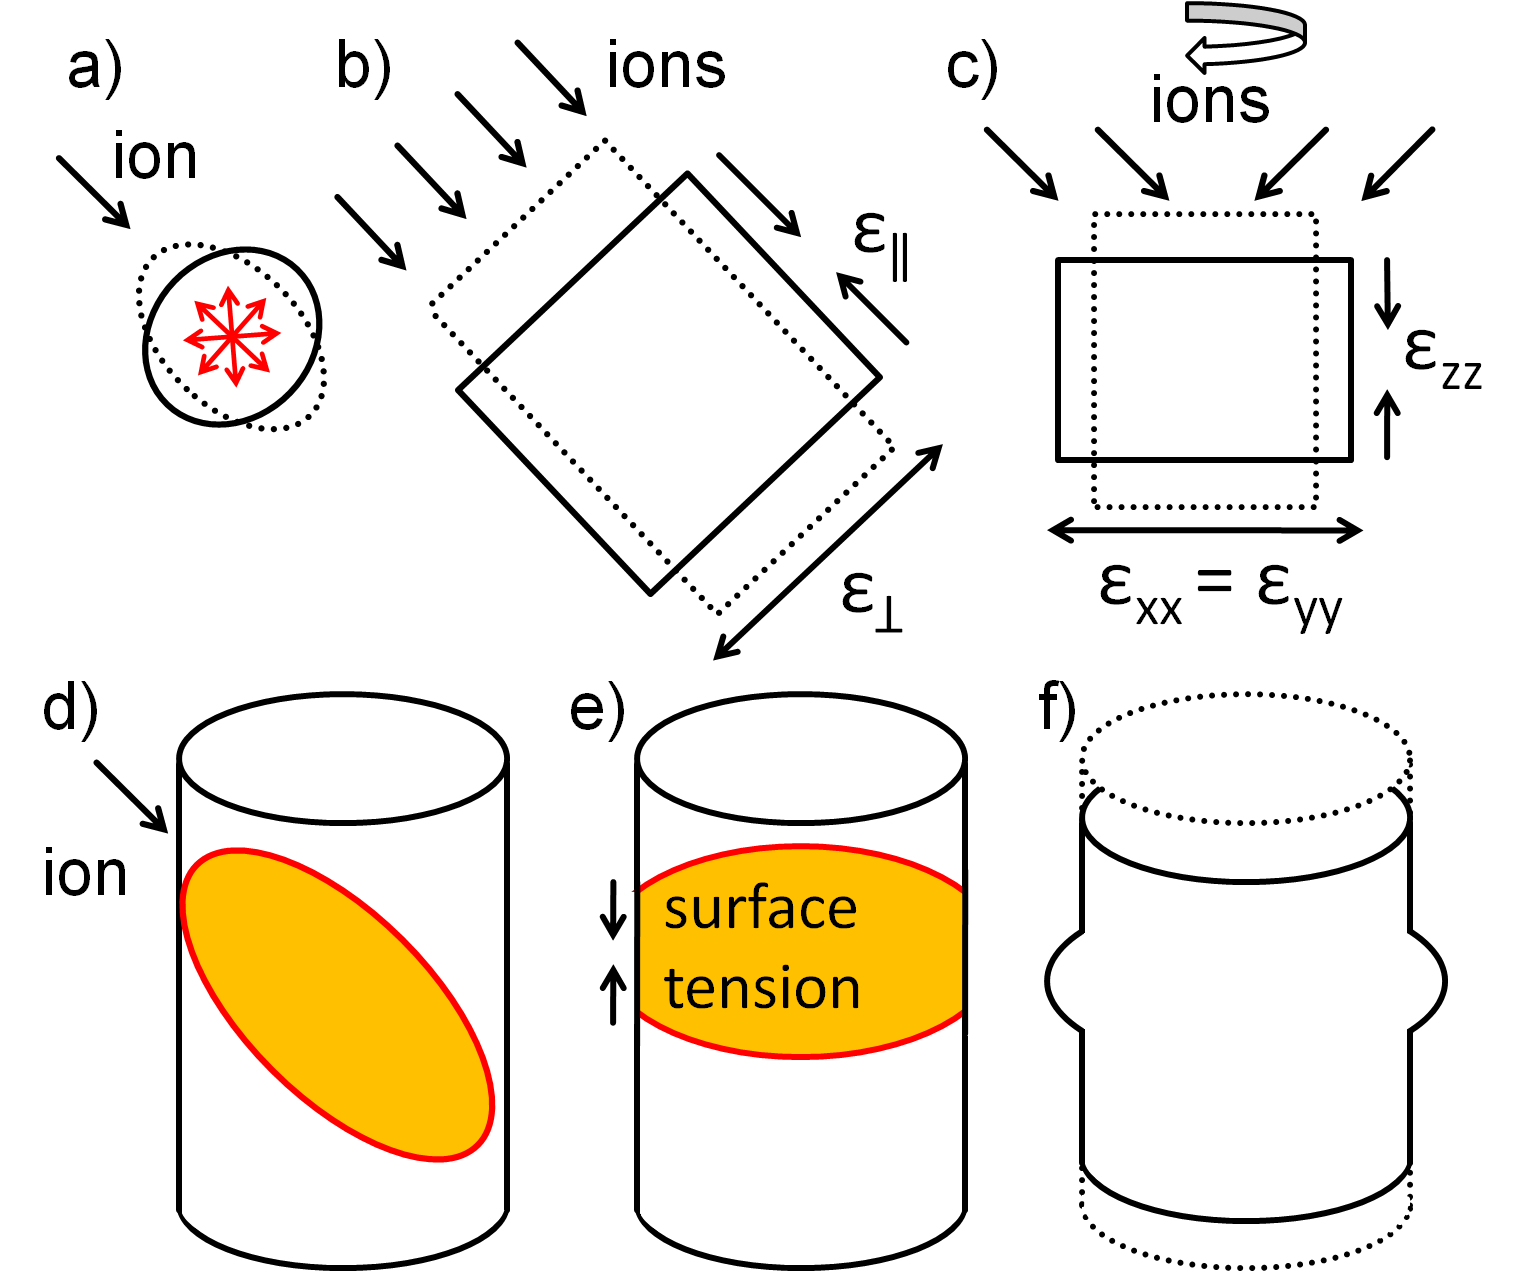
\includegraphics[width=8cm]{images/deformationmodel.jpg}
	\caption{a) - c) Illustration of an deformation model analogous to ion hammering. a) The collision cascade from a single impinging ion heats an approximately ellipsoidal volume of the target material. The internal pressure will lead to an expansion towards a more spherical shape, which is retained upon cooling. b) The net effect of many ions is thus a contraction parallel to and an expansion perpendicular to the ion beam. For no change in density $\epsilon_\parallel = -2\epsilon_\perp$ has to hold. c) Under rotational symmetry this deformation translates to a contraction in the rotational axis $z$ and an expansion in the perpendicular $x-y$ plane with $\epsilon_{zz} = -2\epsilon_{xx} = -\epsilon_\perp$. In d) - f) the alternative, surface tension driven deformation is illustrated. The collision-heated volume of target material shown in d). A significant slice of the wire shown in e) thus has a reduced viscosity. The surface energy is reduced by an increase in the local diameter of the wire, leading to a shortened and thickened wire segment shown in f).} 
	\label{deformationmodel}
\end{figure}

\begin{figure}[htbp]
	\centering
		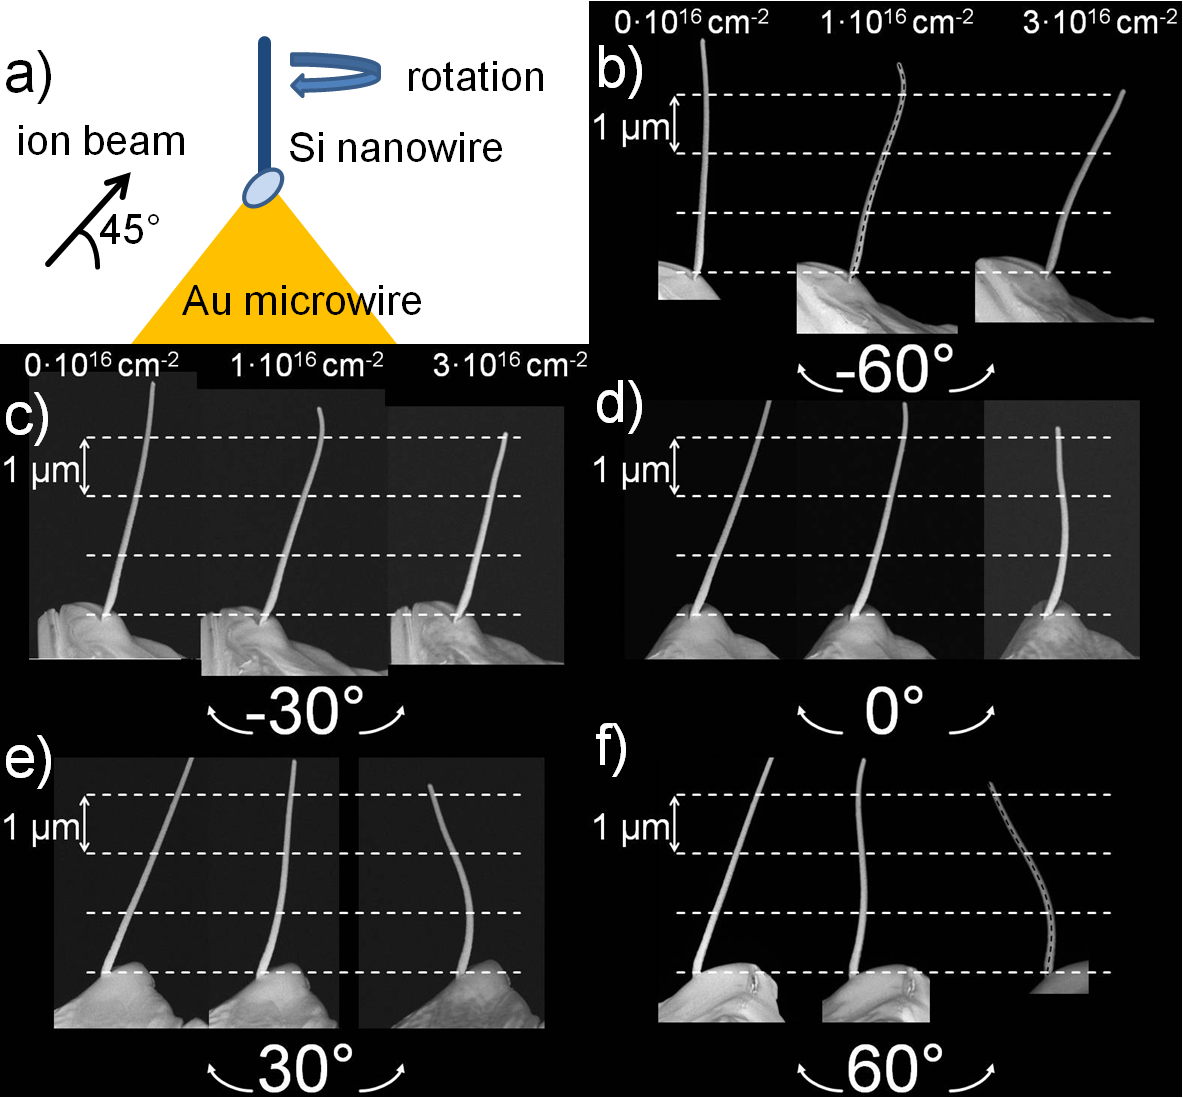
\includegraphics[width=8cm]{images/reverseangle.jpg}
	\caption{ a) Illustration of the nanowire-on-microwire irradiation setup. b) - f) SEM images of the same nanowire as-mounted (left SEM images), after irradiation with $1\times10^{16}\,cm^{-2}$  (center images), and $3\times10^{16}\,cm^{-2}$ (right images) $\,100\,keV Ar^+$ ions. The SEM images where taken with the nanowire rotated by the indicated angle from an angle perpendicular to the angle of rotation. The length of the nanowire after irradiation is determined in b) and f) along the dashed lines.}
	\label{reverseangle}
\end{figure}


\chapter{Summary and Outlook}


\TODO{test}


\bibliography{DissBib}

\end{document}
